\documentclass[10pt]{article}

\usepackage[utf8]{inputenc}
\usepackage{floatrow}


\usepackage{algorithm, algpseudocode}
\let\oldReturn\Return
\renewcommand{\Return}{\State\oldReturn}
\newcommand{\N}{\mathbb{N}}
\newcommand{\R}{\mathbb{R}}

\usepackage[T1]{fontenc}
\usepackage{enumitem}
\usepackage{hyperref}
\usepackage{graphicx}
\usepackage{color}
\usepackage{listings}
\usepackage{wrapfig}
\usepackage{amsmath}
\usepackage{amsfonts}
\usepackage{stmaryrd}
\usepackage{mathtools}
\usepackage[hmargin=1.25in,vmargin=1.25in]{geometry}
\newcommand{\shellcmd}[1]{\\\indent\indent\texttt{\footnotesize\# #1}\\}
  
%title setup
\title{Projet informatique: Honshu (Lot C)}
\author{
  Romain PEREIRA\\
  Douha OURIMI\\
  Afizullah RAHMANY\\
  Guangyue CHEN
}
\date{29/04/2018}

% table of contents setup
\renewcommand{\contentsname}{Sommaire}
\usepackage{etoolbox}
\patchcmd{\thebibliography}{\section*{\refname}}{}{}{}

\hypersetup{
  colorlinks,
  citecolor=black,
  filecolor=black,
  linkcolor=blue,
  urlcolor=red
}

\begin{document}
  \maketitle
  \tableofcontents
  
  \newpage
  \section*{Préambule}
  Ce projet est réalisé dans le cadre de nos études à l'ENSIIE.
  L'objectif est de prendre en main des outils de 'programmation agile',
  en developpant un jeu de carte : le Honshu.
  \newline
  \begin{figure}[H]
    \begin{center}
      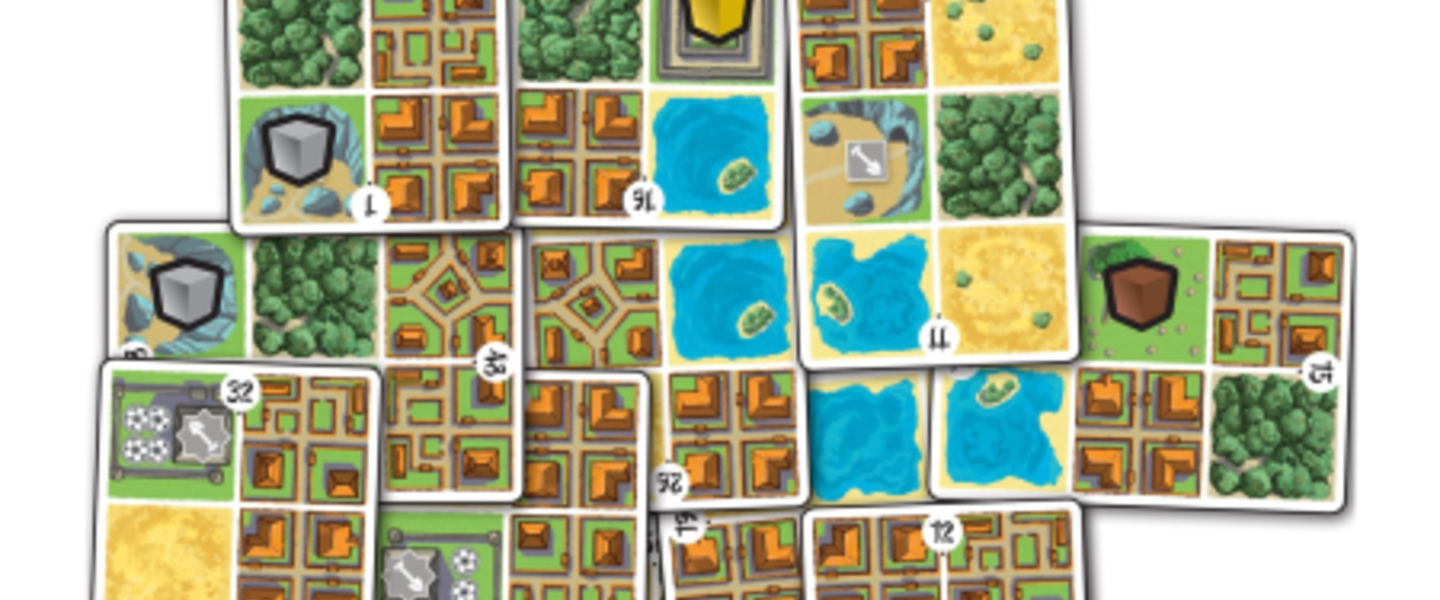
\includegraphics[height=6cm,keepaspectratio]{../images/honshu.png}
    \end{center}
    \caption{\textit{Plateau de jeu}}
    \label{honshu_introduction}
  \end{figure}
  \newpage
  \section{Introduction}
    Pour ce lot, il nous est demandé d'effectuer le calcul des points, et de créer des solveurs (algorithmes proposant une solution de résolution de la grille).
    Le travail a été séparé de la manière suivante:
    \newline
    \newline
    \textit{Douha} : calcul du score
    \newline
    \newline
    \textit{Afizullah} : création de tests unitaires
    \newline
    \newline
    \textit{Romain} et \textit{Guangyue} : création des solveurs (\ref{solveur})
  \section{Calcul du score}
    La fonction de score a été programmé en respectant les règles du sujets.
    (voir 'grille.c')
  \section{Tests unitaires}
    Des tests unitaires ont été implémenté afin de s'assurer que la fonction du calcul de score fonctionne.
    En effet, cette fonction est primordiale pour l'implémentation d'un solveur, c'est pourquoi
    du temps a été consacré à l'élaboration de tests unitaires.
  \section{Interface 'solveur.h'}
    Afin d'avoir une modularité dans notre travail, nous avons normé nos fonctions de solveurs.
    Un solveur prends une grille (tuiles insérés + tuiles en main), et renvoie la liste des insertions
    à effectuer pour obtenir le score trouvé.
    \lstset{language=C}          % Set your language (you can change the language for each code-block optionally)
    \begin{lstlisting}[frame=single]  % Start your code-block
      /** structure qui enregistre une insertion de tuiles */
      typedef struct  s_insertion {
	      /** index de la tuile dans 'grille−>tuiles' */
	      unsigned int tuileID;
	      /** rotation de la tuile */
	      BYTE rotationID;
	      /** position ou la tuile a ete insere */
	      INDEX x, y;
	      /** score après cette insertion */
	      unsigned int score;
      }               t_insertion;

      /** structure qui renvoie le resultat du solveur */
      typedef struct  s_resultat {
	      /** l'ordre dans lequel les tuiles doivent être inseres */
	      t_insertion     * insertion;
	      /** taille du tableau 'insertion' */
	      unsigned int    nb_tuiles;
      }               t_resultat;

      /** typedef d'une fonction de resolution */
      typedef t_resultat * (* t_solveur) (t_grille * grille) ;
    \end{lstlisting}
    \newpage
    \section{Solveur}\label{solveur}
    \subsection{Mise en contexte}
      Afin de mieux envisager les algorithmes suivants, on se propose de travailler dans le cadre suivant.
	\paragraph{Définition}
	On note $G = (M, I)$ une grille, avec:
	\begin{itemize}[label=-]
	  \item $M$ l'ensemble des tuiles en main, $M = \{T_1, ..., T_m\}$, $m = Card(M)$
	  \item $I$ l'ensemble des tuiles insérées sur la grille, $I = \{(T_p, R_p, x_p, y_p, i_p) \slash p \in \{1, ..., k\}\}$, avec
	    \begin{itemize}[label=.]
	      \item $k = Card(I)$
	      \item $T_p$ une tuile
	      \item $R_p$ la rotation de la tuile
	      \item $x_p \in \{1, ..., n\}$ la position $x$ d'insertion de la tuile dans la grille.
	      \item $y_p \in \{1, ..., n\}$ la position $y$ d'insertion de la tuile dans la grille.
	      \item $i_p \in \{1, ..., k\}$ l'indice d'insertion de la tuile sur la grille. (l'ordre dans lequelle elle a été inséré, incrémenteur)
	    \end{itemize}
	\end{itemize}
	On suppose que les n-uplets de $I$ respectent les règles d'insertion.    
	\paragraph{Définition} Une grille $G = (M, I)$ est \textbf{finale} $\Leftrightarrow$ $Card(M) = 0$.
	($\Leftrightarrow$ 'toutes les tuiles sont insérées')
	\paragraph{Définition} Soit $G_1 = (M, I)$ et $G_2 = (N, J)$ 2 grilles.
	On dit que $G_1$ engendre $G_2$ si:
	  \begin{itemize}[label=-]
	    \item $N \subset M$
	    \item $I \subset J$
	    \item $\forall (T, R, x, y, i) \in J \backslash I$, \quad $T \in M \quad et \quad T \notin N$
	  \end{itemize}
	Autrement dit, $G_1$ engendre $G_2$ si l'on peut obtenir $G_2$ en insérant des tuiles de la main de $G_1$.
	
    \subsection{Approche par force brute (parcours en profondeur)}
      Dans un 1er temps, on se propose d'implémenter un algorithme qui renvoie la solution optimale, en effectuant un parcours en profondeur
      sur toutes les combinaisons possibles de grille finale engendrable par une grille donnée.
      \newline
      \newline
      Le problème est le suivant: on suppose que l'on possède une grille de coté $n$, avec $m$ tuiles en main, et $k$ tuiles déjà insérées sur la grille.
      On souhaite tester le score de toutes les configurations possibles de la grille, après insertion des $m$ tuiles en main sur la grille.
      \subsubsection{Etude et expérimentation}
	Experimentalement, (car cela dépends des cases), on remarque la propriété suivante:
	\paragraph{Propriété faible d'insertion}
	Soit $G = (\{T\}, I)$ une grille (avec une seule tuile T en main).
	\newline
	$G$ peut engendrer $\boxed{c * Card(I)}$ grilles finales 2 à 2 distinctes, avec $c \in [10;14]$ une constante d'insertion.
	\newline
	\textbf{N.B}: (voir './complexity.csv'). $c$ semble converger vers $12$ en faisant la moyenne empirique sur des grands échantillons
	de parties aléatoires, mais on se limite à un énoncé faible car la valeur concrete
	de la constante n'a d'intêret que pour l'application numérique finale.
	\paragraph{But} Montrons par récurrence que l'hypothèse $H(m)$ suivante est vrai pour tout $m \in \mathbb{N^*}$.
	\newline
	\newline
	$H(m)$ : pour toute grille $G=(M, I)$, tel que $Card(M) = m \quad et \quad Card(I) = k$,
	G peut engendrer (en moyenne) jusqu'à $\phi(k, m)$ grilles finales 2 à 2 distinctes avec:
	$$\boxed{\phi(k, m) = c^m * \frac{(k + m - 1)!}{(k - 1)!} * m!}$$
	\paragraph{Initialisation}
	Pour $m=1$, d'après la propriété faible d'insertion, on a $\boxed{c * k}$ façon possibles d'insérer la tuile, et:
	  \begin{equation} \label{eq2}
	    \begin{split}
	      \phi(k, m) & = c^m * \frac{(k + m - 1)!}{(k - 1)!} * m! \\
			& = c^1 * \frac{(k + 1 - 1)!}{(k - 1)!} * 1! \\
			& = c * \frac{k!}{(k - 1)!} * 1 \\
			& = c * k
	    \end{split}
	  \end{equation}
	  Donc $H(G)$ est vérifié pour toute grille $G=(M, I)$ tel que $Card(M) = m = 1$.
	\paragraph{Récurrence}
	  On suppose $H(G)$ vraie pour toute grille $G=(M, I)$ tel que $Card(M) \leq m$.
	  \newline
	  Montrons que $H(m+1)$ est vraie.
	  \newline
	  Soit $G=(M, I)$ une grille tel que $$Card(M)=m+1\quad et \quad Card(I)=k\ quelconque$$
	  D'après la propriété faible d'insertion, $G$ peut engendrer jusqu'à $c*k*(m+1)$
	  grille $G'=(I', M')$ tel que $Card(I') = k + 1$ et $Card(M') = m$.
	  Par hypothèse de récurrence, chaque $G'$ peut engendrer jusqu'à $\phi(k + 1, m)$ grilles.
	  Le nombre de grilles finales engendrables par $G$ est donc de:
	  \begin{equation} \label{eq3}
	    \begin{split}
	      c * k * (m + 1) * \phi(k, m) & = c * k * (m + 1) * c^m * \frac{(k + m - 1)!}{(k - 1)!} * m! \\
					  & = c^{m + 1} * k * \frac{(k + m - 1)!}{(k - 1)!} * (m + 1)! \\
					  & = c^{m + 1} * \frac{(k + m)!}{(k - 1)!} * (m + 1)! \\
					  & = \boxed{\phi(k, m + 1)}
	    \end{split}
	  \end{equation}
	  La récurrence est vérifiée.
	\paragraph{Conclusion}
	  Une grille $G=(M, I)$ peut engendrer en moyenne jusqu'à $\phi(k, m)$ grilles finales.

	\paragraph{Complexité du parcours en profondeur}
	  Le calcul du score est un algorithme en $O(n^2)$.
	  Trouver les insertions a effectué sur une grille G, afin d'obtenir un score optimal à l'aide d'un parcours en profondeur,
	  est donc effectué avec une complexité
	  $$\boxed{C(k, m, n) = \phi(k, m) * O(n^2)}$$
	
	\paragraph{Application numérique}
	  On se place dans le cadre du sujet: on possède une grille $$G=(M, I)\ tel\ que \quad Card(M)=m \quad et \quad Card(I)=k=1$$
	  \begin{equation} \label{eq1}
	    \begin{split}
	      \phi(k, m) & = c^m * \frac{(k + m - 1)!}{(k - 1)!} * m! \\
			& = c^m * \frac{(1 + m - 1)!}{(1 - 1)!} * m! \\
			& = c^m * (m!)^2 \\
	    \end{split}
	  \end{equation}
	  On choisit $c = 12$.
	  \newline
	  En fonction de $m$, on obtient donc un nombre de grille final engendrable de:
	  \begin{itemize}[label=-]
	    \item $m=1 \Rightarrow \phi(k, m) = 12$
	    \item $m=2 \Rightarrow \phi(k, m) = 576$
	    \item $m=3 \Rightarrow \phi(k, m) = 62\ 208$
	    \item $m=4 \Rightarrow \phi(k, m) = 11\ 943\ 936$
	  \end{itemize}
	  Soit pour une grille de coté $n=32$, un nombre d'opération élémentaire de l'ordre de:
	  \begin{itemize}[label=-]
	    \item $m=1 \Rightarrow C(k, m, n) = 12288$
	    \item $m=2 \Rightarrow C(k, m, n) = 589\ 824$
	    \item $m=3 \Rightarrow C(k, m, n) = 63\ 700\ 992$
	    \item $m=4 \Rightarrow C(k, m, n) = 12\ 230\ 590\ 464$
	  \end{itemize}
	  On remarque que très rapidement, lorsque $m$ augmente, cette approche (par force brute $\Leftrightarrow$ parcours en profondeur)
	  est beaucoup trop lourde temporellement.
	  Cependant, elle nous permettra d'assurer l'optimalité du résultat pour des petites grilles,
	  afin de comparer ses résultats avec les algorithmes futurs.
	  \paragraph{Remarque}
	  Dans l'implémentation final, l'algorithme de score a été optimisé: on ne parcourt plus les $n^2$ cases de la grille,
	  mais on garde en mémoire la position la plus 'en haut à gauche', et la plus 'en bas à droite' d'une case non vide,
	  et on ne vérifie que le rectangle formé par ces 2 points.
      \newpage
      \subsubsection{Algorithme}
	\begin{algorithm}
	  \caption{Renvoie le score optimal atteignable pour une grille donnée}
	  \begin{algorithmic}[1]
	    \Function{parcours\_en\_profondeur}{$G=(M, I)$}
	      \Function{parcourir}{$G=(M, I)$, $best$}
		\For{$T \in M$}
		  \For{$R \in \{NORD, SUD, EST, OUEST\}$}
		    \For{$x \in \{1, ..., n\}$}
		      \For{$y \in \{1, ..., n\}$}
			\If{$(T, R, x, y)$ peut être inséré dans $I$}
			  \State (Insérer) : supprimer $T$ de $M$ et ajouter $(T, R, x, y)$ à $I$
			  \State (Vérifier optimalité)
			  \If{$Card(M) = 0$}
			    \State $best := \mathtt{max}(best, \mathtt{score}(G))$
			  \Else
			    \State $best := \mathtt{parcourir}(G, best)$
			  \EndIf
			  \State (Dé-insérer) : ajouter $T$ à $M$ et supprimer $(T, R, x, y)$ de $I$
			\EndIf
		      \EndFor
		    \EndFor
		  \EndFor
		\EndFor
		\Return $best$
	      \EndFunction
	      \Return $parcourir(G, 0)$
	    \EndFunction
	  \end{algorithmic}
	\end{algorithm}
    \newpage
    \subsection{Approche par algorithme glouton}
      Dans une seconde approche, on se propose de créer un algorithme glouton. Bien que l'on perdra l'optimalité globale,
      on garde un résultat localement optimal, pour une complexité moins lourde qu'avec le parcours en profondeur.
      \subsubsection{Algorithme}
      	L'algorithme glouton fonctionne sur le principe suivant: pour une grille donnée, insérer toutes les tuiles une à une,
	en insérant à chaque tour le n-uplet (tuile, rotation, x, y) maximisant le score.
	\begin{algorithm}
	  \caption{Renvoie un score localement optimal pour une grille donnée}
	  \begin{algorithmic}[1]
	    \Function{glouton}{$G=(M, I)$}
	      \While{$M \neq \emptyset$}
		\State $bestLocalScore := 0$
		\State $bestTuile := (T=0, R=0, x=0, y=0)$
		\For{$T \in M$}
		  \For{$R \in \{NORD, SUD, EST, OUEST\}$}
		    \For{$x \in \{1, ..., n\}$}
		      \For{$y \in \{1, ..., n\}$}
			\If{$(T, R, x, y)$ peut être inséré dans $I$}
			  \State (Insérer) : supprimer $T$ de $M$ et ajouter $(T, R, x, y)$ à $I$
			  \State (Vérifier optimalité local)
			  \If {$bestLocalScore < \mathtt{score}(G)$}
			    \State $bestLocalScore := \mathtt{score}(G)$
			    \State $bestTuile := (T, R, x, y)$
			  \EndIf
			  \State (Dé-insérer) : ajouter $T$ à $M$ et supprimer $(T, R, x, y)$ de $I$
			\EndIf
		      \EndFor
		    \EndFor
		  \EndFor
		\EndFor
		\State (Insérer optimum local) : supprimer $T$ de $M$ et ajouter $(T, R, x, y)$ à $I$
	      \EndWhile
	    \EndFunction
	  \end{algorithmic}
	\end{algorithm}
	\newline
	Cet algorithme a une complexité:
	\begin{equation} \label{eq1}
	  \begin{split}
	    C(n, m) & = \sum_{k=1}^{m}{4*n^2*c*k} \\
		    & = 4cn^2 \sum_{k=1}^{m}{k} \\
		    & = 4cn^2 \frac{m(m+1)}{2} \\
		    & \boxed{\simeq 2cn^2m^2}
	  \end{split}
	\end{equation}
      \newpage
      \subsubsection{Experimentation}
	Les fichiers '.csv' correspondant aux données d'études sont disponibles dans ce même dossier.
	\begin{figure}[H]
	  \begin{center}
	    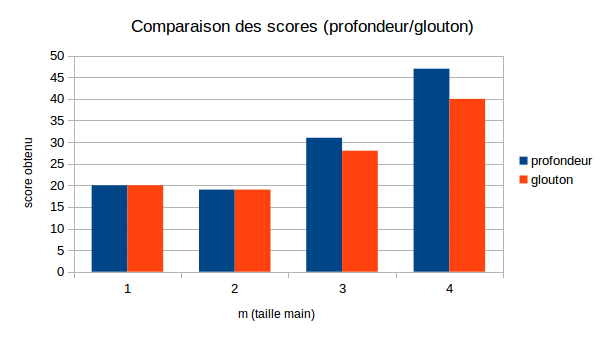
\includegraphics[height=6cm,keepaspectratio]{./comparaison.png}
	  \end{center}
	  \caption{\textit{Comparaison des scores obtenus entre les 2 algorithmes}}
	\end{figure}
	\textbf{N.B}: L'algorithme de parcours en profondeur étant trop lents, la comparaison n'a pas pu être effectué pour des valeurs plus grandes de $m$.
	
  	\begin{figure}[H]
	  \begin{center}
	    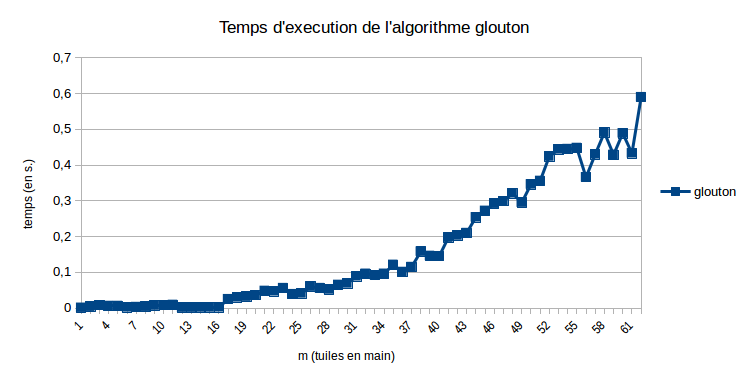
\includegraphics[height=6cm,keepaspectratio]{./glouton.png}
	  \end{center}
	  \caption{\textit{Temps d'execution de la résolution par algorithme glouton, en fonction du nombre de tuiles en main: complexité quadratique en $m$}}
	\end{figure}
	
	\paragraph{Remarque} Une comparaison temporelle des 2 algorithmes n'est pas pertinente, car l'algorithme en profondeur explose temporellement.
	Voici quelques valeurs qui ont pu être obtenus:
	\begin{itemize}[label=-]
	  \item $m=1$ ; profondeur: $0.001 s.$ ; glouton: $0.001 s.$
	  \item $m=2$ ; profondeur: $0.007 s.$ ; glouton: $0.004 s.$
	  \item $m=3$ ; profondeur: $1.314 s.$ ; glouton: $0.008 s.$
	  \item $m=4$ ; profondeur: $131.6 s.$ ; glouton: $0.006 s.$
	\end{itemize}
      \subsection{Conclusion}
	Ce document rapporte donc une étude et une comparaison de 2 algorithmes standarts de résolution: une approche par parcours en profondeur,
	et une approche par algorithme glouton.
	\paragraph{PS.1}
	Une piste de résolution, qui n'a pas été exploité par manque de temps, est un mixage des 2 méthodes.
	Dans l'algorithme glouton, l'optimalité local est assuré sur chaques insertions.
	Une autre approche (plus lente) aurait consister à assurer l'optimalité sur $x$ insertions.
	On insère les tuiles par paquet de $x$ tuiles, et de manière optimal en faisant un parcours en profondeur 'local' sur $x$ insertions.
	\paragraph{Remarque} Pour $x=1$, on retrouve l'algorithme glouton, pour $x=m$ on retrouve l'algorithme de parcours en largeur.
	\newline
	\newline
	Malheureusement, cette approche n'a pas été implementé et étudié par manque de temps.
	De plus, au regard des performances du parcours en largeur, seule les valeurs $x=2$ ou $x=3$ aurait été possibles.
	
	\paragraph{PS.2}
	Une autre approche a été implémenté mais non-étudié / approfondie par manque de temps.
	Cette approche se base sur un parcours en profondeur, mais avec une fonction \textit{filtre}.
	Ce \textit{filtre} a pour but de limiter la profondeur du parcours: lorsque l'on remarque qu'une insertion
	ne satisfait pas les contraintes du filtre, le parcours s'arrête pour cette branche.
	Pour un filtre judicieusement choisit, on peut alors obtenir de meilleurs scores qu'avec l'algorithme glouton,
	pour un temps de recherche raisonnable. (plus lent que l'algorithme glouton, mais plus rapide que l'approche sans filtre)
    \newpage
  \section{Conclusion}
    Pour ce lot, le travail a été séparé de manière efficace, et la plupart du code a ainsi pu être programmé pendant la séance encadré.
    La résolution de ce type de problème (NP-difficle) a déjà été étudié en IPF (dans le projet SUBSET\_SUM) pour Romain, Douha et Guangyue.
    Les différentes approches s'en sont inspirés (naïve, glouton, naïve avec filtre...).
    Ce sont des méthodes de résolutions classiques de problèmes NP-difficiles.
\end{document}
